\documentclass[12pt,a4paper]{scrbook}
\usepackage[utf8]{inputenc}
\usepackage[ngerman]{babel}
\usepackage{graphicx}
\usepackage{geometry}
\geometry{left=2.00cm, right=2.00cm, top=2.00cm, bottom=2.00cm}
\pagestyle{empty}

\usepackage[bf]{caption}
\newcommand{\Abb}[1]{\textbf{Abbildung \ref{#1}}}

\begin{document}
\chapter{Testkapitel}
\section{Testabschnitt}
\subsection{Testunterabschnitt}
\clearpage

\Abb{fig:house} zeigt das Haus vom Nikolaus. 
\begin{figure}[htb]
	\centering
	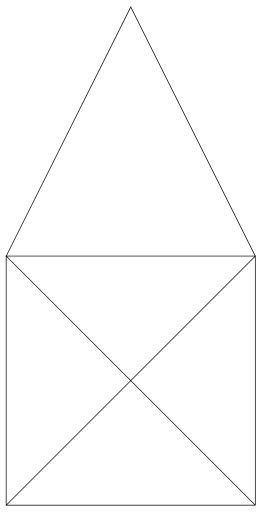
\includegraphics[width=2cm]{house/house.png}
	\caption{Das Haus}
	\label{fig:house}
\end{figure}

\renewcommand{\figurename}{Bild}
\renewcommand{\Abb}[1]{\textit{\figurename~\ref{#1}}}
\captionsetup{labelfont=it}

\Abb{fig:house} zeigt das Haus vom Nikolaus. 
\begin{figure}[htb]
	\centering
	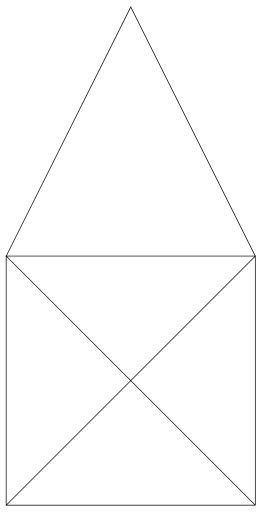
\includegraphics[width=2cm]{house/house.png}
	\caption{Das Haus}
	\label{fig:house2}
\end{figure}

\end{document}